\subsection{Stochastic Bandit}

Using the methods metioned in \ref{sec:stochastic_bandit_method}, the relationship between average regret and the number of rounds for different trajectory-generation methods and algorithms is presented in Figure \ref{fig:stochastic_bandit_pretrained} and Table \ref{table:stochastic_bandit_pretrained}. Each experiment was run for 50000 rounds and repeated 100 times; the regret from each run was averaged cumulatively, and this average is reported as the final result.

\begin{figure}[htbp]
    \centering
    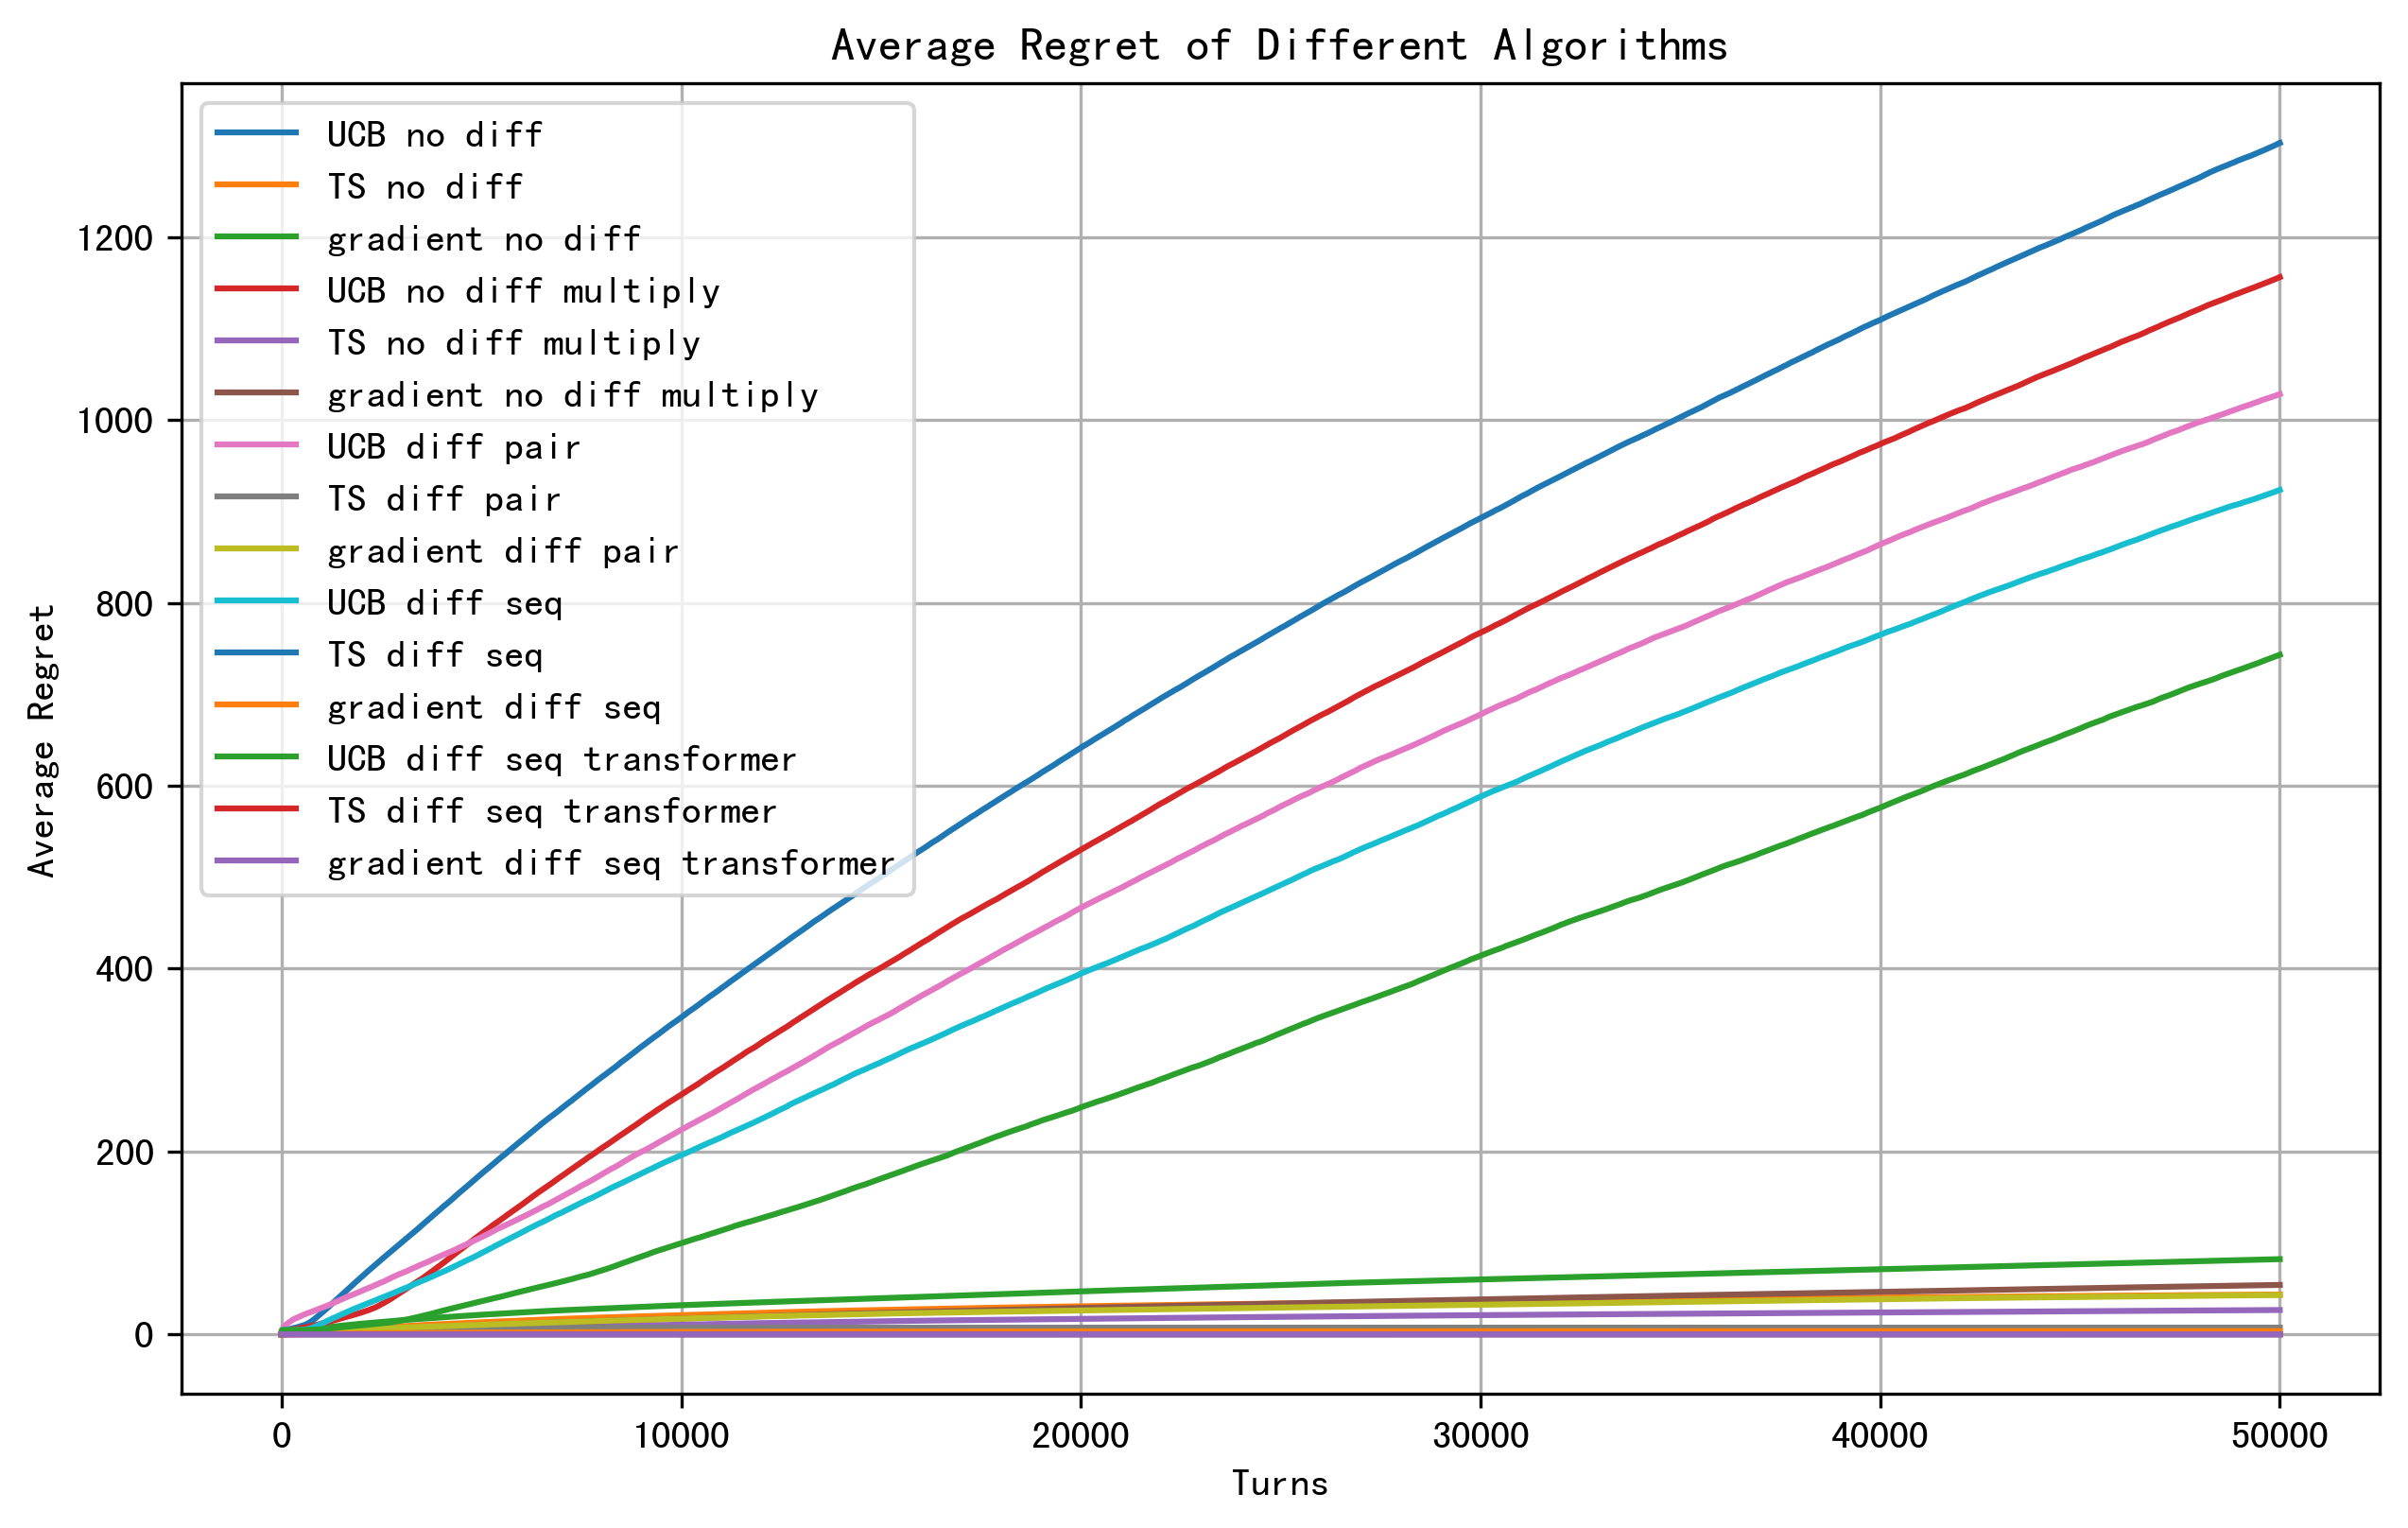
\includegraphics[width=\textwidth]{./Img/stochastic_bandit/pretrain.png}
    \caption{Average cumulative-regret curves for the UCB algorithm (UCB), Thompson Sampling (TS), and the policy-gradient algorithm (gradient) under five data settings: the unaugmented offline dataset (no diff), a duplicated-concatenated version of the original dataset (no-diff-multiply), tuple-level discrete-diffusion augmentation (diff pair), sequence-level discrete-diffusion augmentation (diff seq), and Transformer-based sequence discrete-diffusion augmentation (diff seq transformer).}
    \label{fig:stochastic_bandit_pretrained}
\end{figure}

\begin{table}[htbp]
    \centering
    \begin{tabular}{c c c c}
    \toprule
    Trajectory generation policy & UCB & TS & policy gradient \\
    \midrule
    no offline dataset & 1691.827 & 163.483 & 858.794 \\
    offline, no enlarge & 1303.405 & 43.550  & 82.254 \\
    offline+copy & 1156.635 & 26.596  & 54.048 \\
    offline+diffuse pair & 1028.613 & 7.296 & 42.993 \\
    offline+diffusion sequence & 923.779 & 0.071 & 3.522 \\
    offline+diffusion sequence (Transformer) & 743.441 & 0.008 & 0.002 \\
    \bottomrule
\end{tabular}
\caption{Performance(average accumulated regret) of various algorithms on Bernoulli-reward bandits under different offline-dataset enlargement (trajectory-generation) policies.}
\label{table:stochastic_bandit_pretrained}
\end{table}

We observe that both Thompson Sampling and the policy-gradient algorithm achieve lower regret than UCB. With effective trajectory augmentation, the two methods essentially identify the optimal arm, driving the cumulative regret toward zero. To verify that a discrete-diffusion model can generate additional useful trajectories and thereby improve UCB as well, we varied the amount of synthetic data used for pre-training. All synthetic trajectories were produced with the most effective method identified earlier—the Transformer-based sequence discrete-diffusion model—generating an extra 100, 500, and 1000 trajectories. As baselines of the same sizes, the original (non-diffusion) dataset was duplicated once, five times, and ten times, respectively. Following the same algorithmic procedure, the resulting average-regret curves over rounds for the different generation strategies and algorithms are reported in Figure \ref{fig:stochastic_bandit_num} and Table \ref{table:stochastic_bandit_num}. Each experiment consisted of 50000 rounds, repeated 100 times; the regret values from each run were averaged to obtain the final results.

\begin{figure}[htbp]
    \centering
    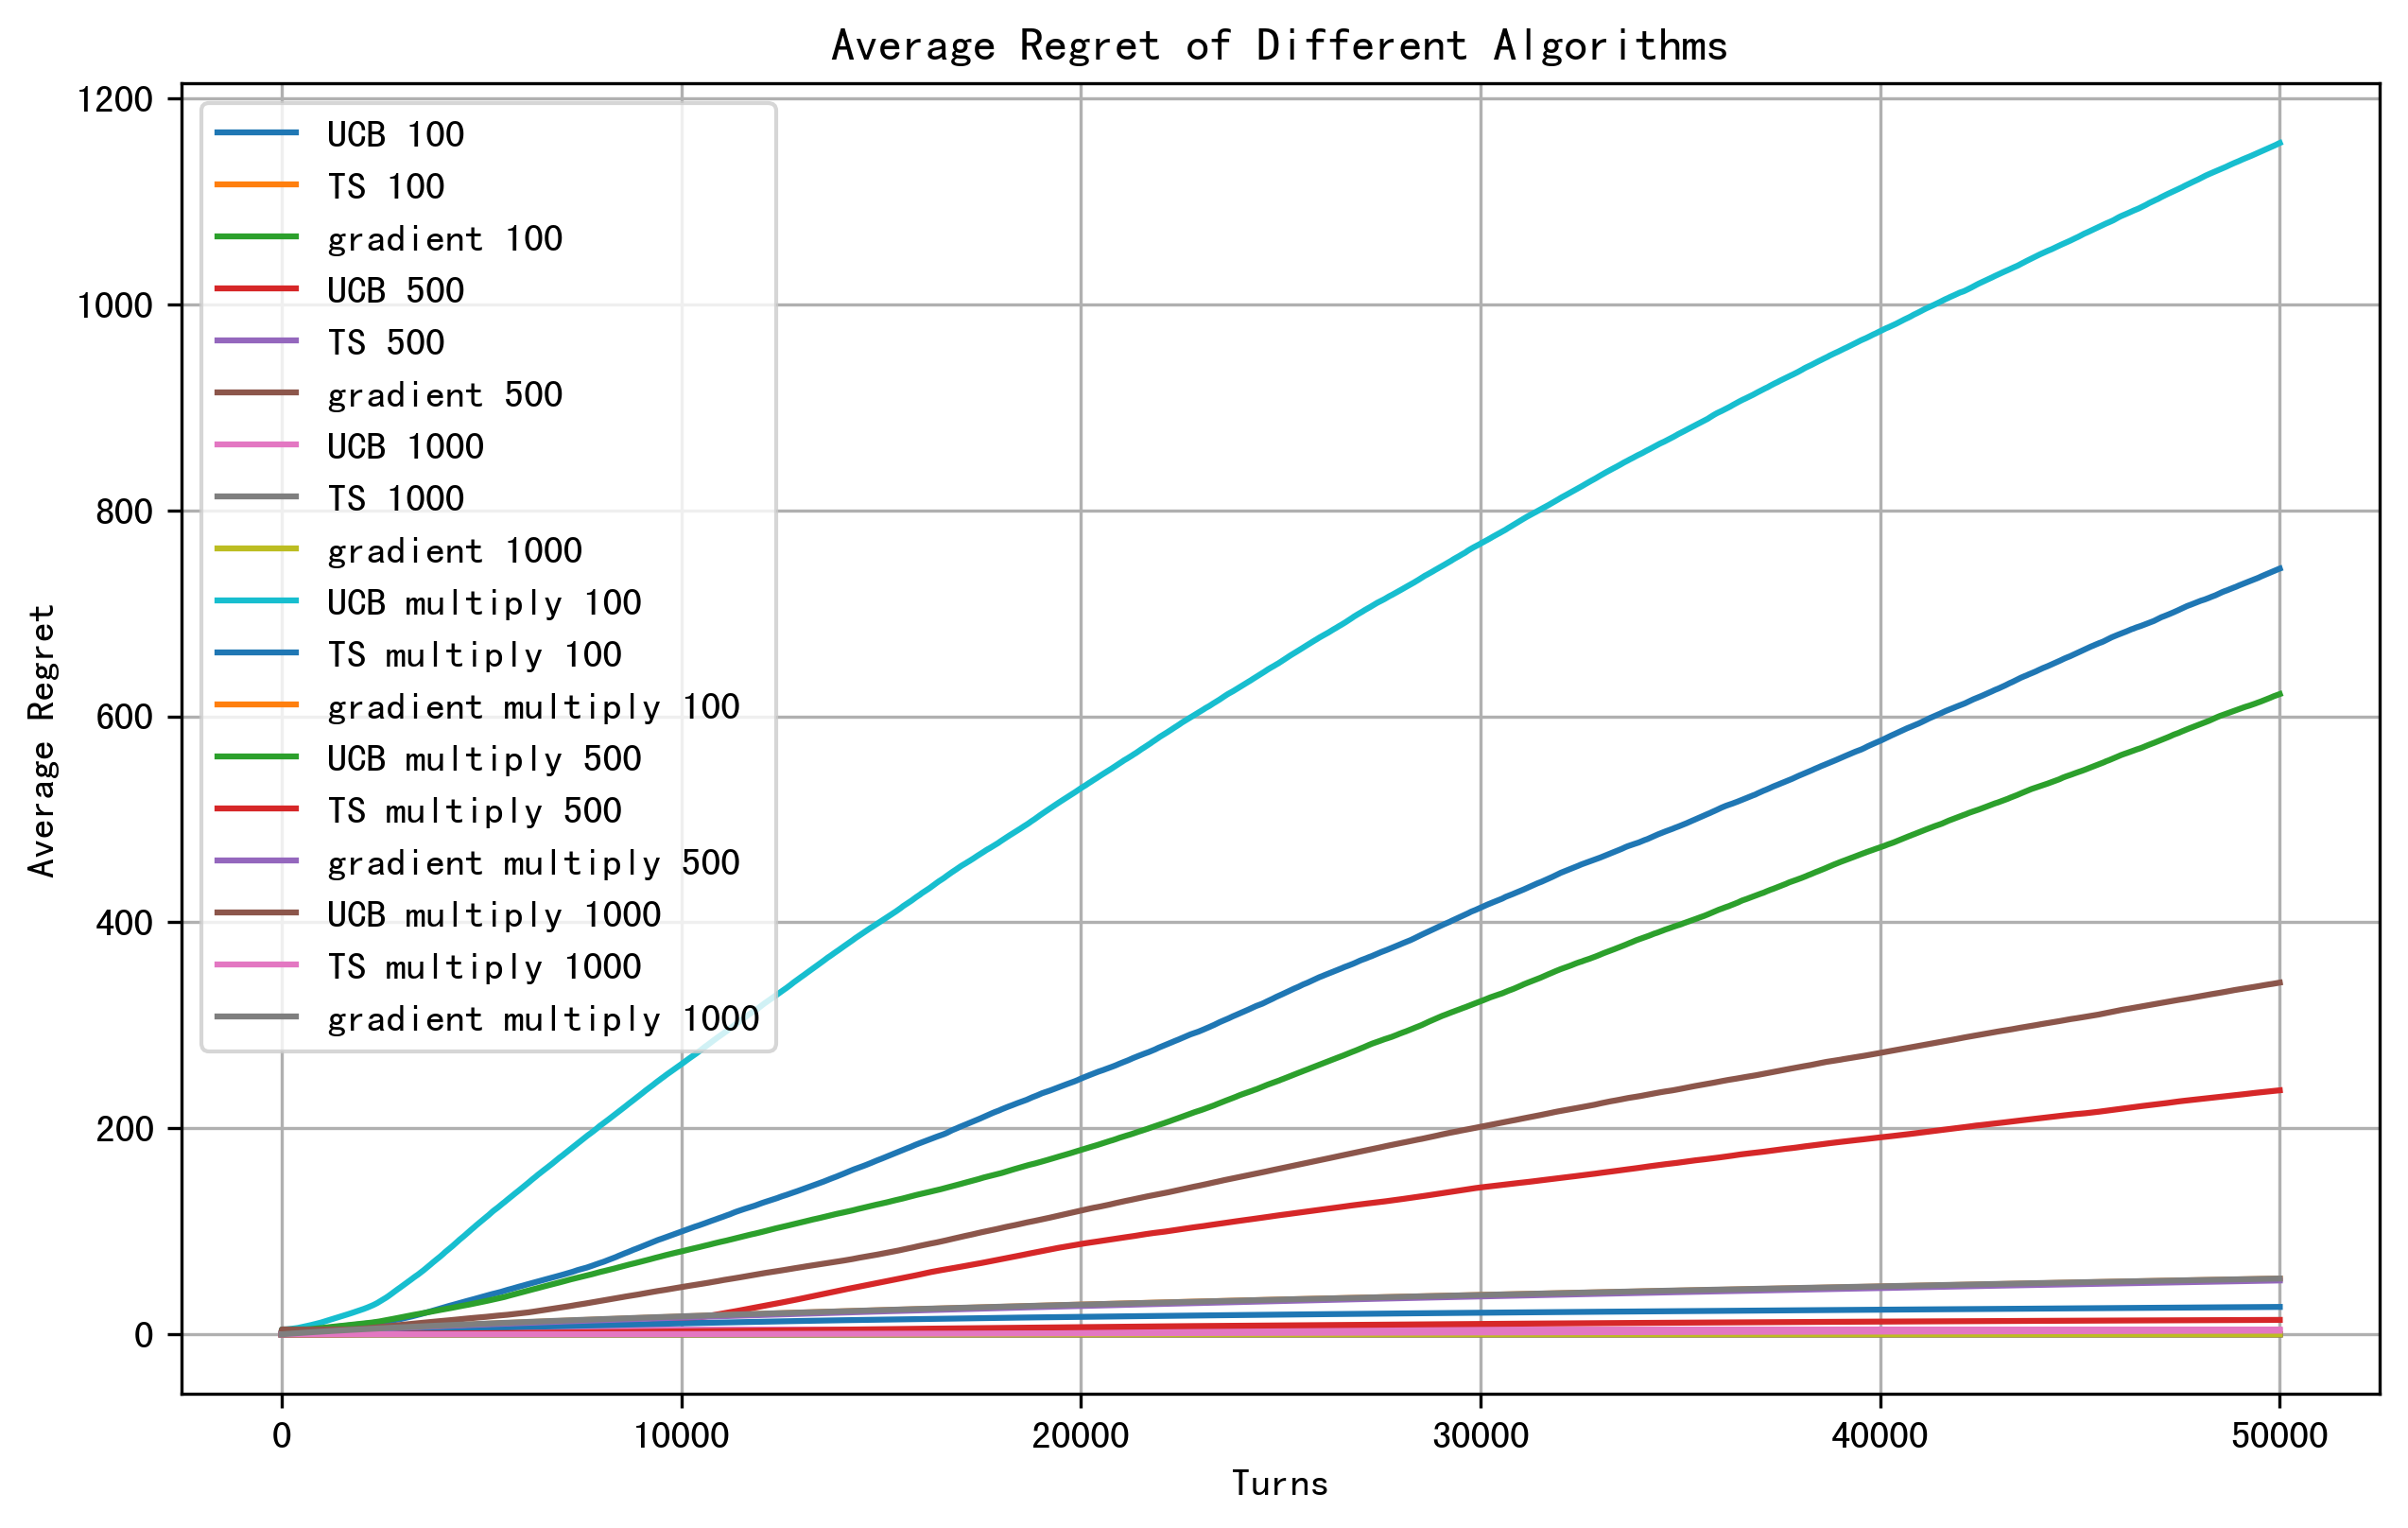
\includegraphics[width=\textwidth]{./Img/stochastic_bandit/time_comparison.png}
    \caption{Average cumulative-regret curves for the UCB algorithm (UCB), Thompson Sampling (TS), and the gradient bandit (gradient) under six data regimes: Transformer-based sequence discrete-diffusion augmentation with 100, 500, and 1 000 additional trajectories (100, 500, 1000) and simple duplication of the original dataset yielding the same numbers of extra trajectories (multiply 100, multiply 500, multiply 1000).}
    \label{fig:stochastic_bandit_num}
\end{figure}

\begin{table}[htbp]
    \centering
    \begin{tabular}{c c c c}
    \toprule
    Trajectory generation policy & UCB & TS & policy gradient \\
    \midrule
    copy, 100 trajectories& 1156.635 & 26.596 & 54.048 \\
    copy, 500 trajectories& 621.581 & 13.996 & 52.293 \\
    copy, 1000 trajectories & 341.470 & 3.517 & 54.164 \\
    diffusion, 100 trajectories & 743.441 & 0.008 & 0.002 \\
    diffusion, 500 trajectories & 236.908 & 0.056 & 0.000 \\
    diffusion, 1000 trajectories & 4.660 & 0.025 & 0.000 \\
    \bottomrule
\end{tabular}
\caption{Performance(average accumulated regret) of various algorithms on Bernoulli-reward bandits under different offline-dataset enlargement (trajectory-generation) policies.}
\label{table:stochastic_bandit_num}
\end{table}

The experimental results indicate that, under identical settings, enlarging the number of trajectories produced by the discrete diffusion model yields substantial gains for all three algorithms—UCB, Thompson Sampling, and the gradient bandit. In particular, both Thompson Sampling and the gradient method converge rapidly once pre-training is introduced, driving their cumulative regret close to zero and underscoring the pivotal role of pre-training in policy learning. The UCB algorithm likewise benefits markedly: its performance improves steadily as more synthetic trajectories are added. A further comparison confirms the effectiveness of discrete diffusion for generating high-quality data: when the number of additional trajectories is held constant, datasets augmented by diffusion outperform those expanded by simply duplicating and concatenating the original logs, demonstrating superior practical utility and generalisation capacity in data-augmentation scenarios.


To evaluate the method’s adaptability under non-ideal reward conditions, we construct a discrete-reward environment in which each arm follows a Bernoulli distribution. Under this setting, Thompson Sampling no longer enjoys a convenient conjugate prior and thus cannot be applied directly. Instead, trajectories are generated by running the UCB algorithm online with the environment, collecting 100 trajectories of length 50. The reward variable is defined as follows:
$$X=\begin{cases}
0 & \text{ w.p. } \theta_1 \\
0.5 & \text{ w.p. } \theta_2 \\
1 & \text{ w.p. } 1-\theta_1-\theta_2 \\
\end{cases}$$

Under three arm-count configurations (20, 25, and 30), we systematically evaluated the effect of diffusion-generated trajectories on the pre-training phase of these algorithms to assess the method’s generalization capability in high-complexity policy spaces.

The discrete diffusion method that demonstrated the best performance under Bernoulli rewards was used to generate 500 additional trajectories. We compared three pre-training strategies: no pre-training, pre-training on the original offline dataset, and pre-training on the offline dataset augmented with these 500 diffusion-generated trajectories. Both the UCB algorithm and a policy-gradient method were evaluated. Following this procedure, the evolution of average regret over rounds for each trajectory-generation method and algorithm is presented in Figure \ref{fig:non_bern} and Table \ref{table:non_bern}. Each experiment ran for 50 000 rounds and was repeated 100 times; the reported results are the average regret across all trials.

\begin{figure}[htbp]
    \centering
    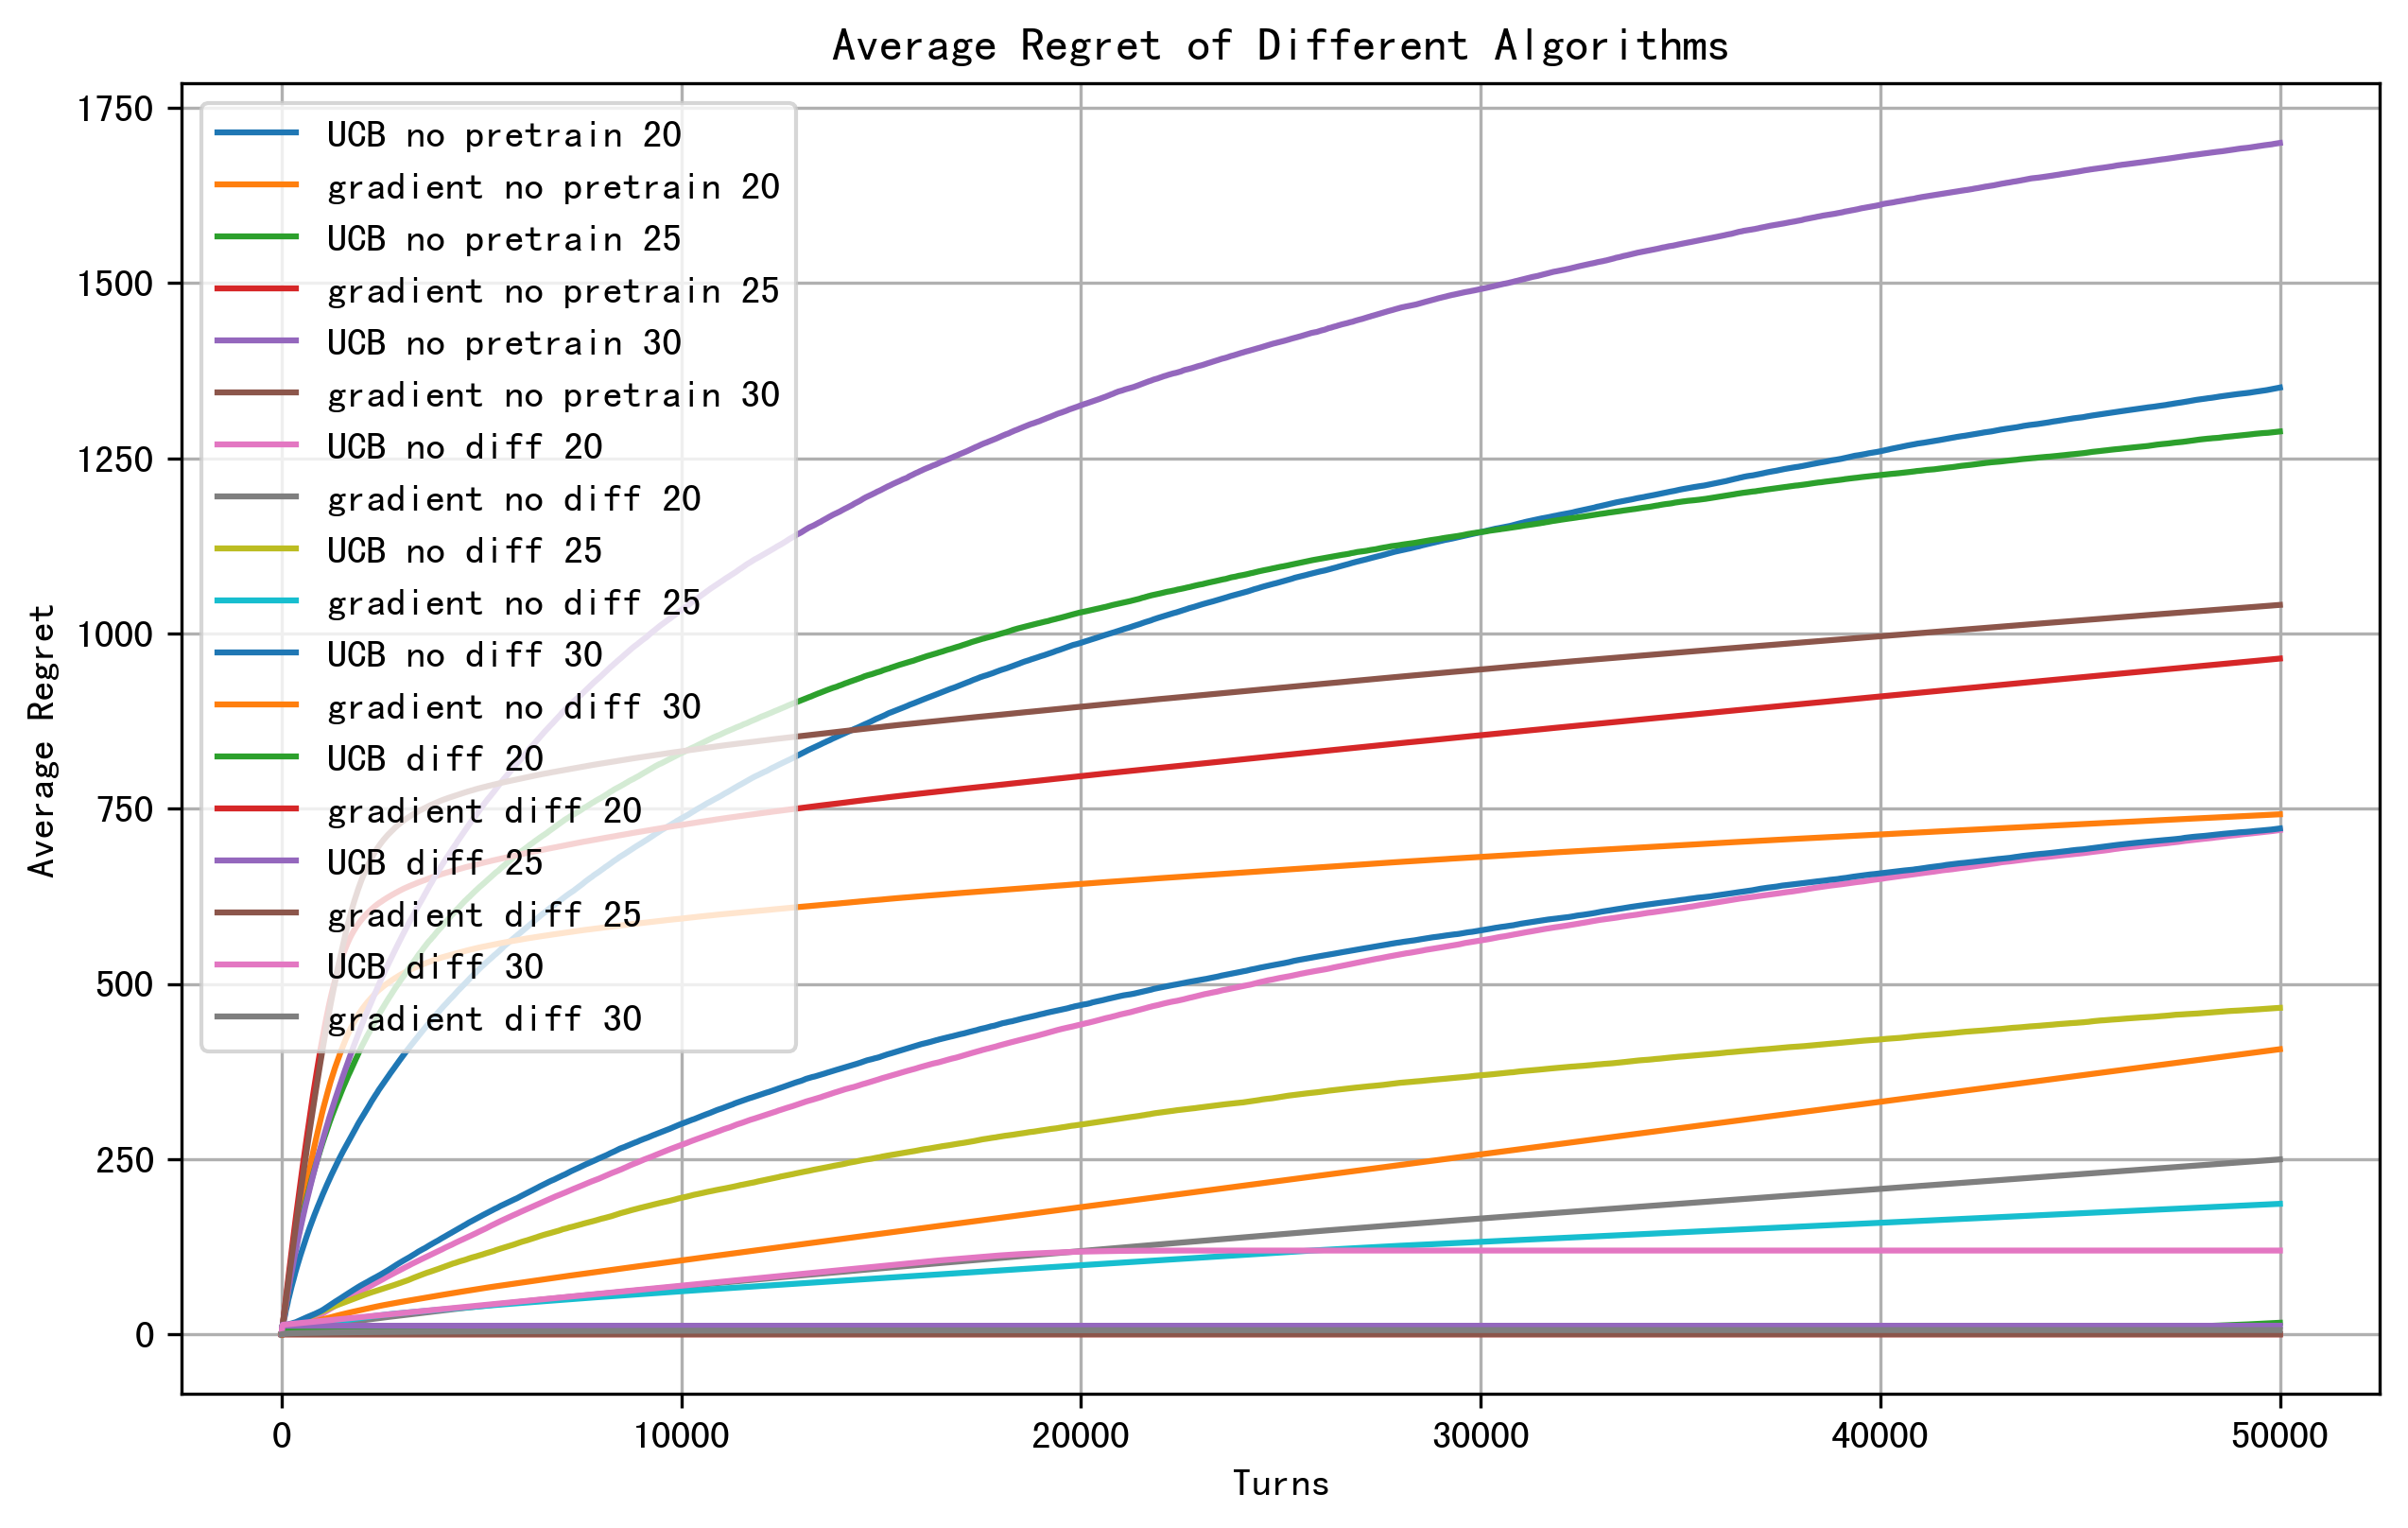
\includegraphics[width=0.97\textwidth]{./Img/stochastic_bandit/non_bern.png}
    \caption{Average cumulative-regret curves for the UCB algorithm (UCB) and the policy-gradient algorithm (Gradient) under nine configurations formed by three arm counts (20, 25, and 30) and three pre-training regimes: no pretraining (no pretrain), pretraining on the original dataset without diffusion (no diff), and pretraining on a dataset augmented with trajectories generated by the Transformer-based sequential discrete diffusion method (diff).}
    \label{fig:non_bern}
\end{figure}

\begin{table}[htbp]
    \centering
    \begin{tabular}{c c c}
    \toprule
    Trajectory generation policy & UCB & policy gradient \\
    \midrule
    no offline dataset, 20 arms & 1351.033 & 742.086 \\
    offline, no enlarge, 20 arms & 719.629 & 249.610 \\
    offline+diffusion sequence (Transformer), 20 arms & 16.517 & 0.000 \\
    no offline dataset, 25 arms & 1288.369 & 964.330 \\
    offline, no enlarge, 25 arms & 465.870 & 186.230 \\
    offline+diffusion sequence (Transformer), 25 arms & 12.220 & 0.000 \\
    no offline dataset, 30 arms & 1700.104 & 1040.903 \\
    offline, no enlarge, 30 arms & 721.866 & 406.857 \\
    offline+diffusion sequence (Transformer), 30 arms & 119.548 & 6.077 \\
    \bottomrule
\end{tabular}
\caption{Performance(average accumulated regret) of various algorithms on Bernoulli-reward bandits under different offline-dataset enlargement (trajectory-generation) policies.}
\label{table:non_bern}
\end{table}

The experimental results indicate that in discrete-reward environments with non-Bernoulli distributions, using UCB-generated online interaction data as trajectories and augmenting the offline dataset via a discrete diffusion model enables both the policy-gradient algorithm and the UCB algorithm to achieve effective performance with 20, 25, and 30 arms. Moreover, as the number of arms increases, a larger volume of trajectory data is required to accurately learn each arm’s reward function.

Since the policy‐gradient algorithm and the gradient bandit algorithm share similar implementations but rest on different principles, we conducted experiments to verify that, when supplied with an offline dataset, the policy‐gradient method yields superior performance. Both algorithms were evaluated under various offline data regimes, and the evolution of their average regret over rounds is shown in Figure \ref{fig:compare_gradient_bandit} and Table \ref{table:compare_gradient_bandit}. Each experiment comprised 50000 rounds and was repeated 100 times; the reported results are the average regret across all runs.

\begin{figure}[htbp]
    \centering
    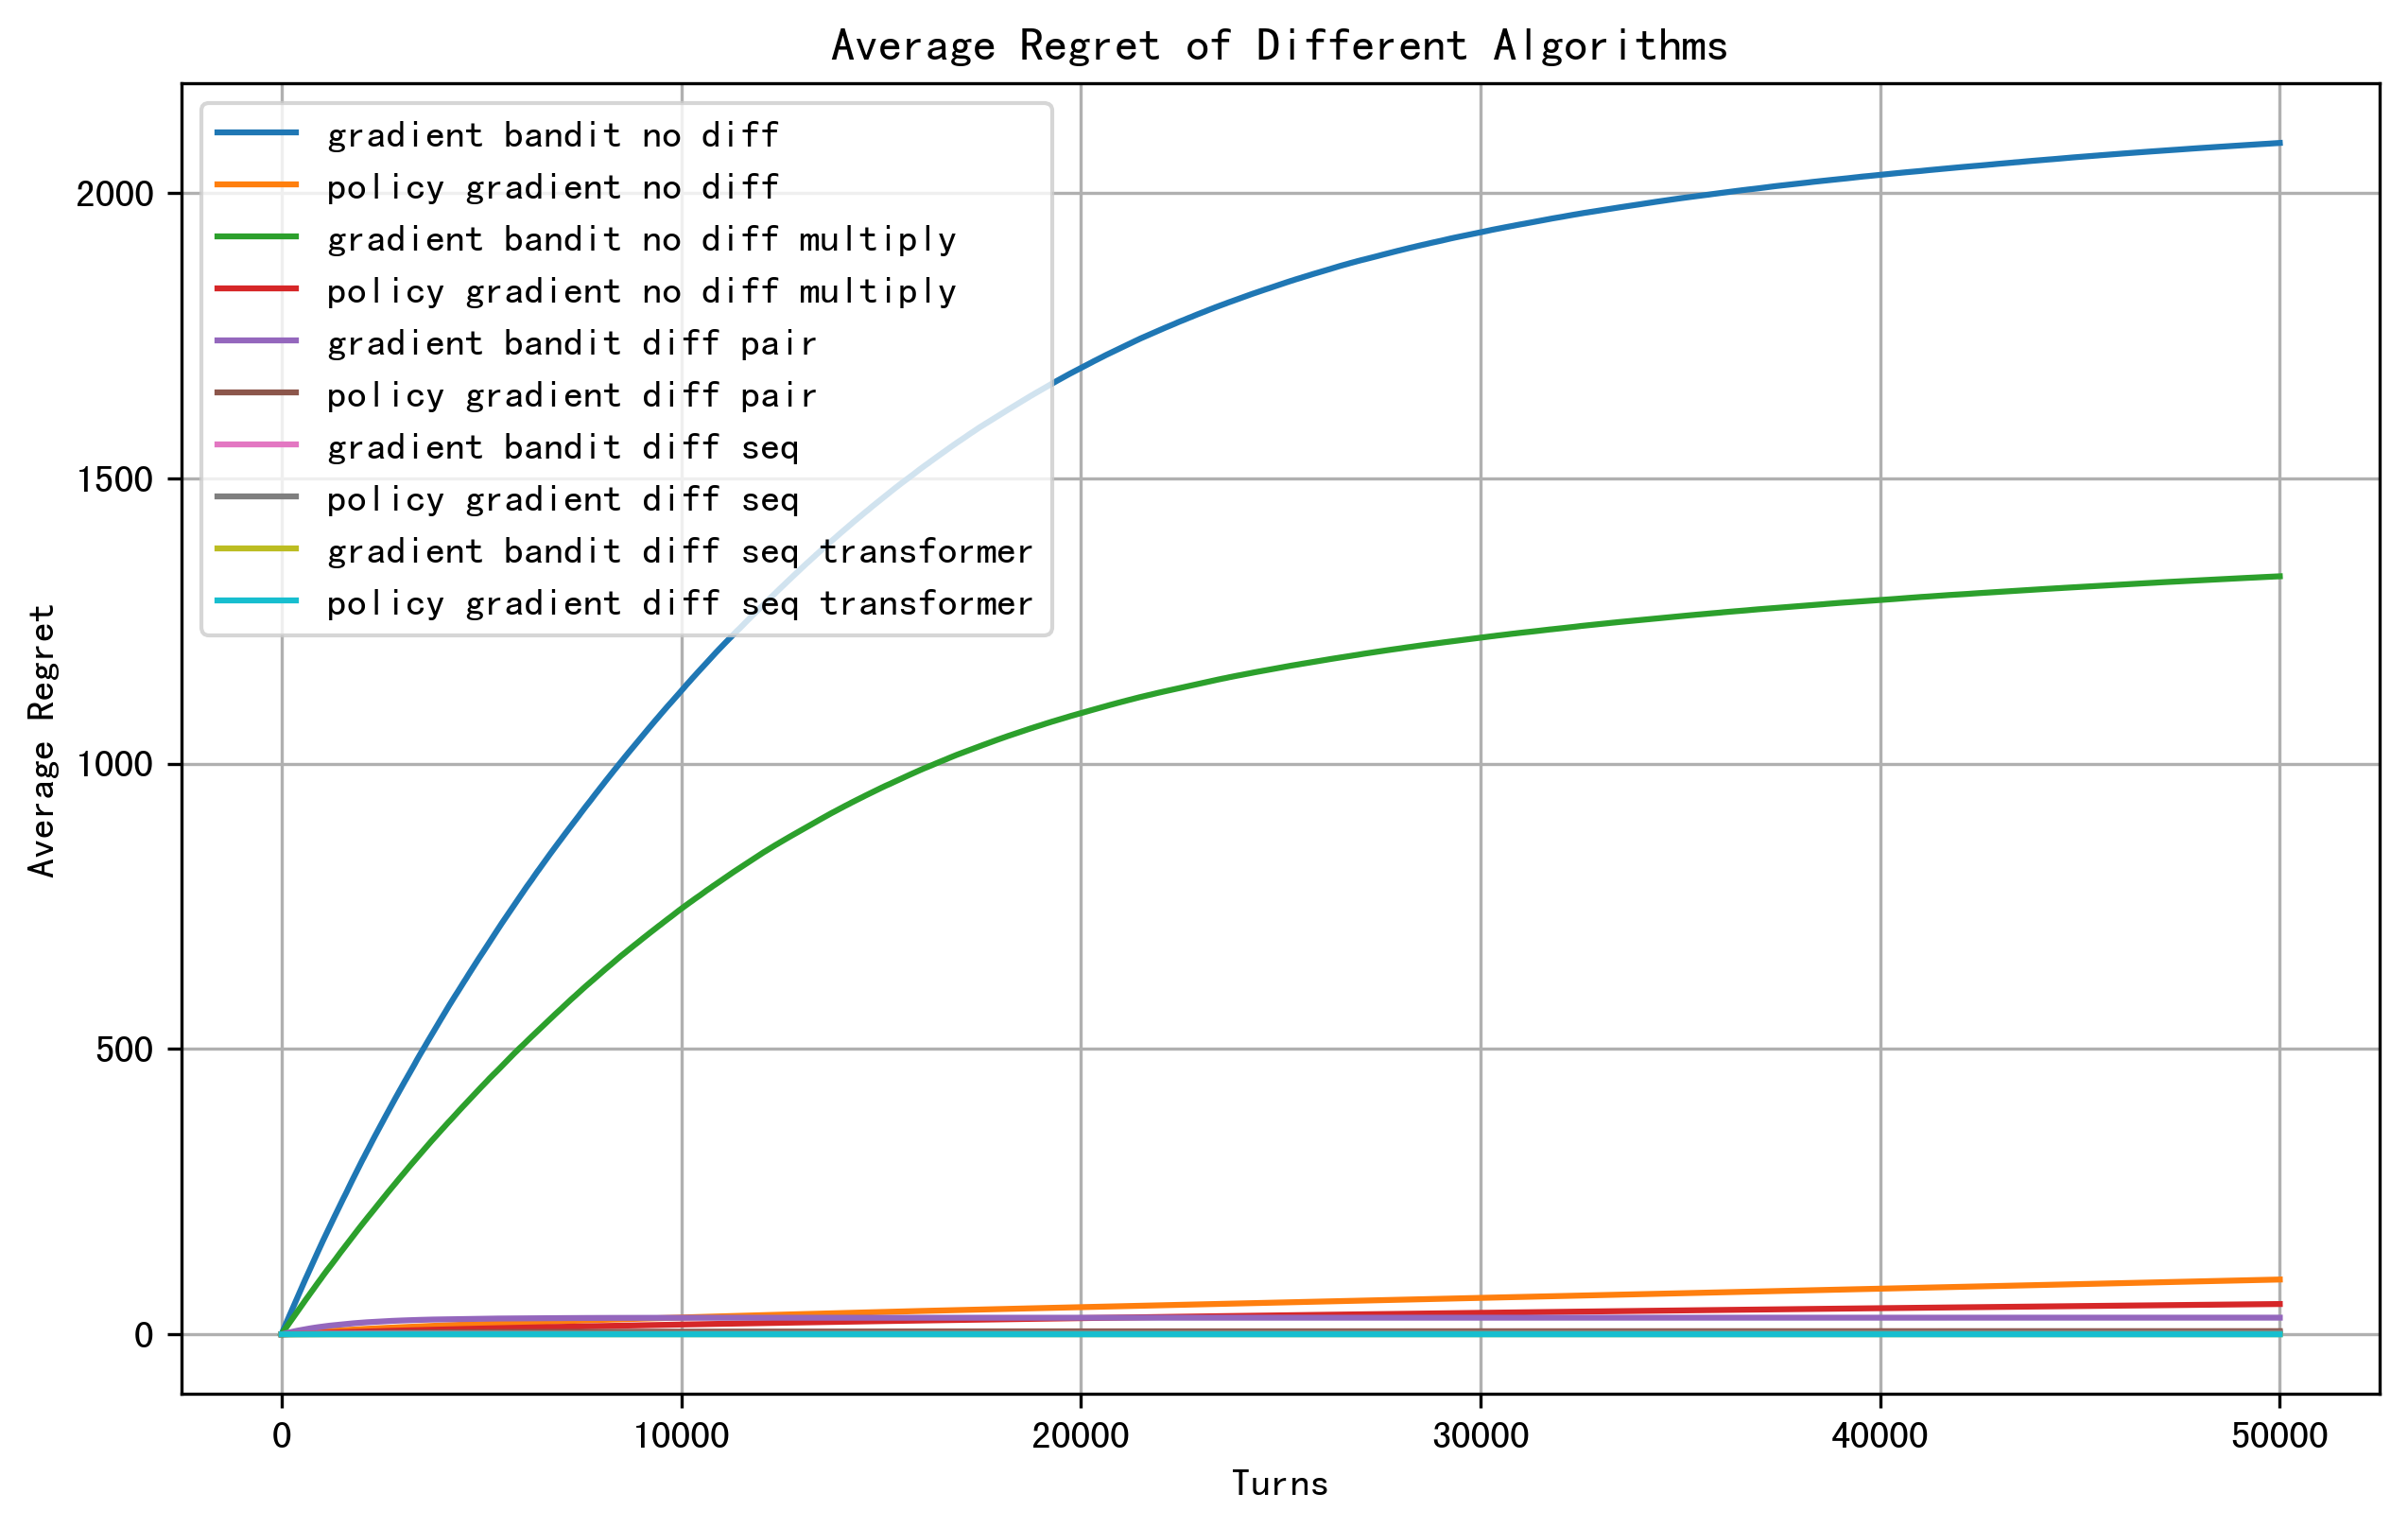
\includegraphics[width=0.9\textwidth]{./Img/stochastic_bandit/compare_gradient_bandit.png}
    \caption{Average cumulative-regret curves for the policy-gradient algorithm (Policy Gradient) and the gradient-bandit algorithm (Gradient Bandit) under five data regimes: the raw offline dataset without augmentation (no diff), the original dataset duplicated and concatenated (no diff multiply), tuple-level discrete diffusion augmentation (diff pair), sequential discrete diffusion augmentation (diff seq), and Transformer-based sequential discrete diffusion augmentation (diff seq transformer).}
    \label{fig:compare_gradient_bandit}
\end{figure}

\begin{table}[htbp]
    \centering
    \begin{tabular}{c c c}
    \toprule
    Trajectory generation policy & policy gradient & gradient bandit \\
    \midrule
    offline, no enlarge & 96.010 & 2078.776 \\
    offline+copy & 53.095 & 1316.211 \\
    offline+diffuse pair & 5.500 & 34.418 \\
    offline+diffusion sequence & 2.629 & 1.712 \\
    offline+diffusion sequence (Transformer) & 0.001 & 0.140 \\
    \bottomrule
\end{tabular}
\caption{Performance(average accumulated regret) of various algorithms on Bernoulli-reward bandits under different offline-dataset enlargement (trajectory-generation) policies.}
\label{table:compare_gradient_bandit}
\end{table}

Additionally, to confirm that the generated trajectories accurately capture the true distribution, we plot in Figure \ref{fig:distribution} both the number of times each arm is selected and each arm’s average observed reward. Because arms with higher indices have larger expected rewards in our setting, they are sampled more frequently, as expected. Moreover, the empirical mean reward for each arm closely matches its true expectation, demonstrating the effectiveness of our trajectory‐generation method.

\begin{figure}[htbp]
    \centering
    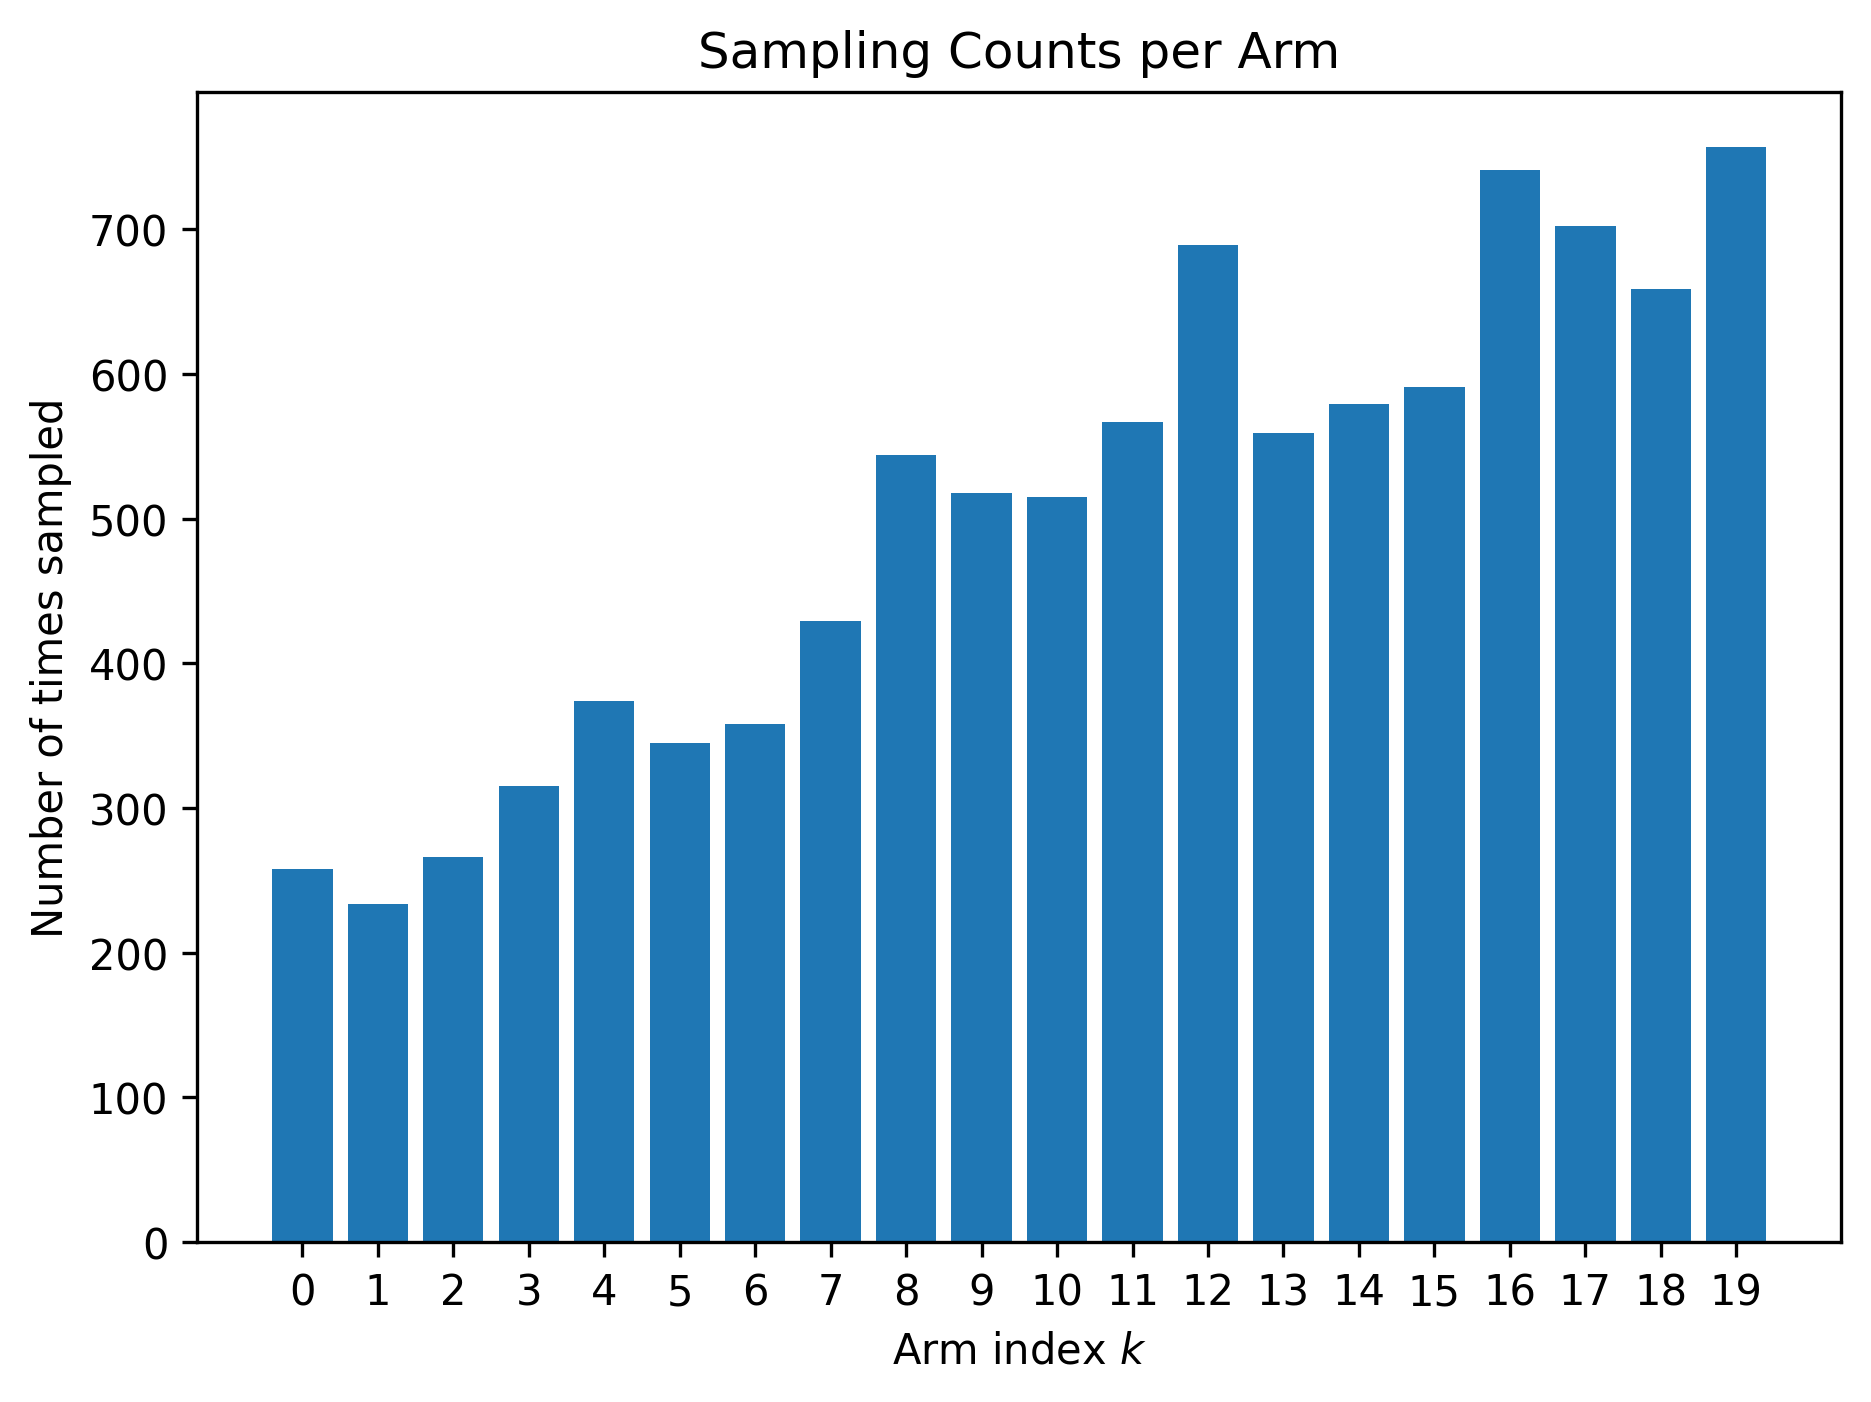
\includegraphics[width=0.48\textwidth]{./Img/stochastic_bandit/count.png}
    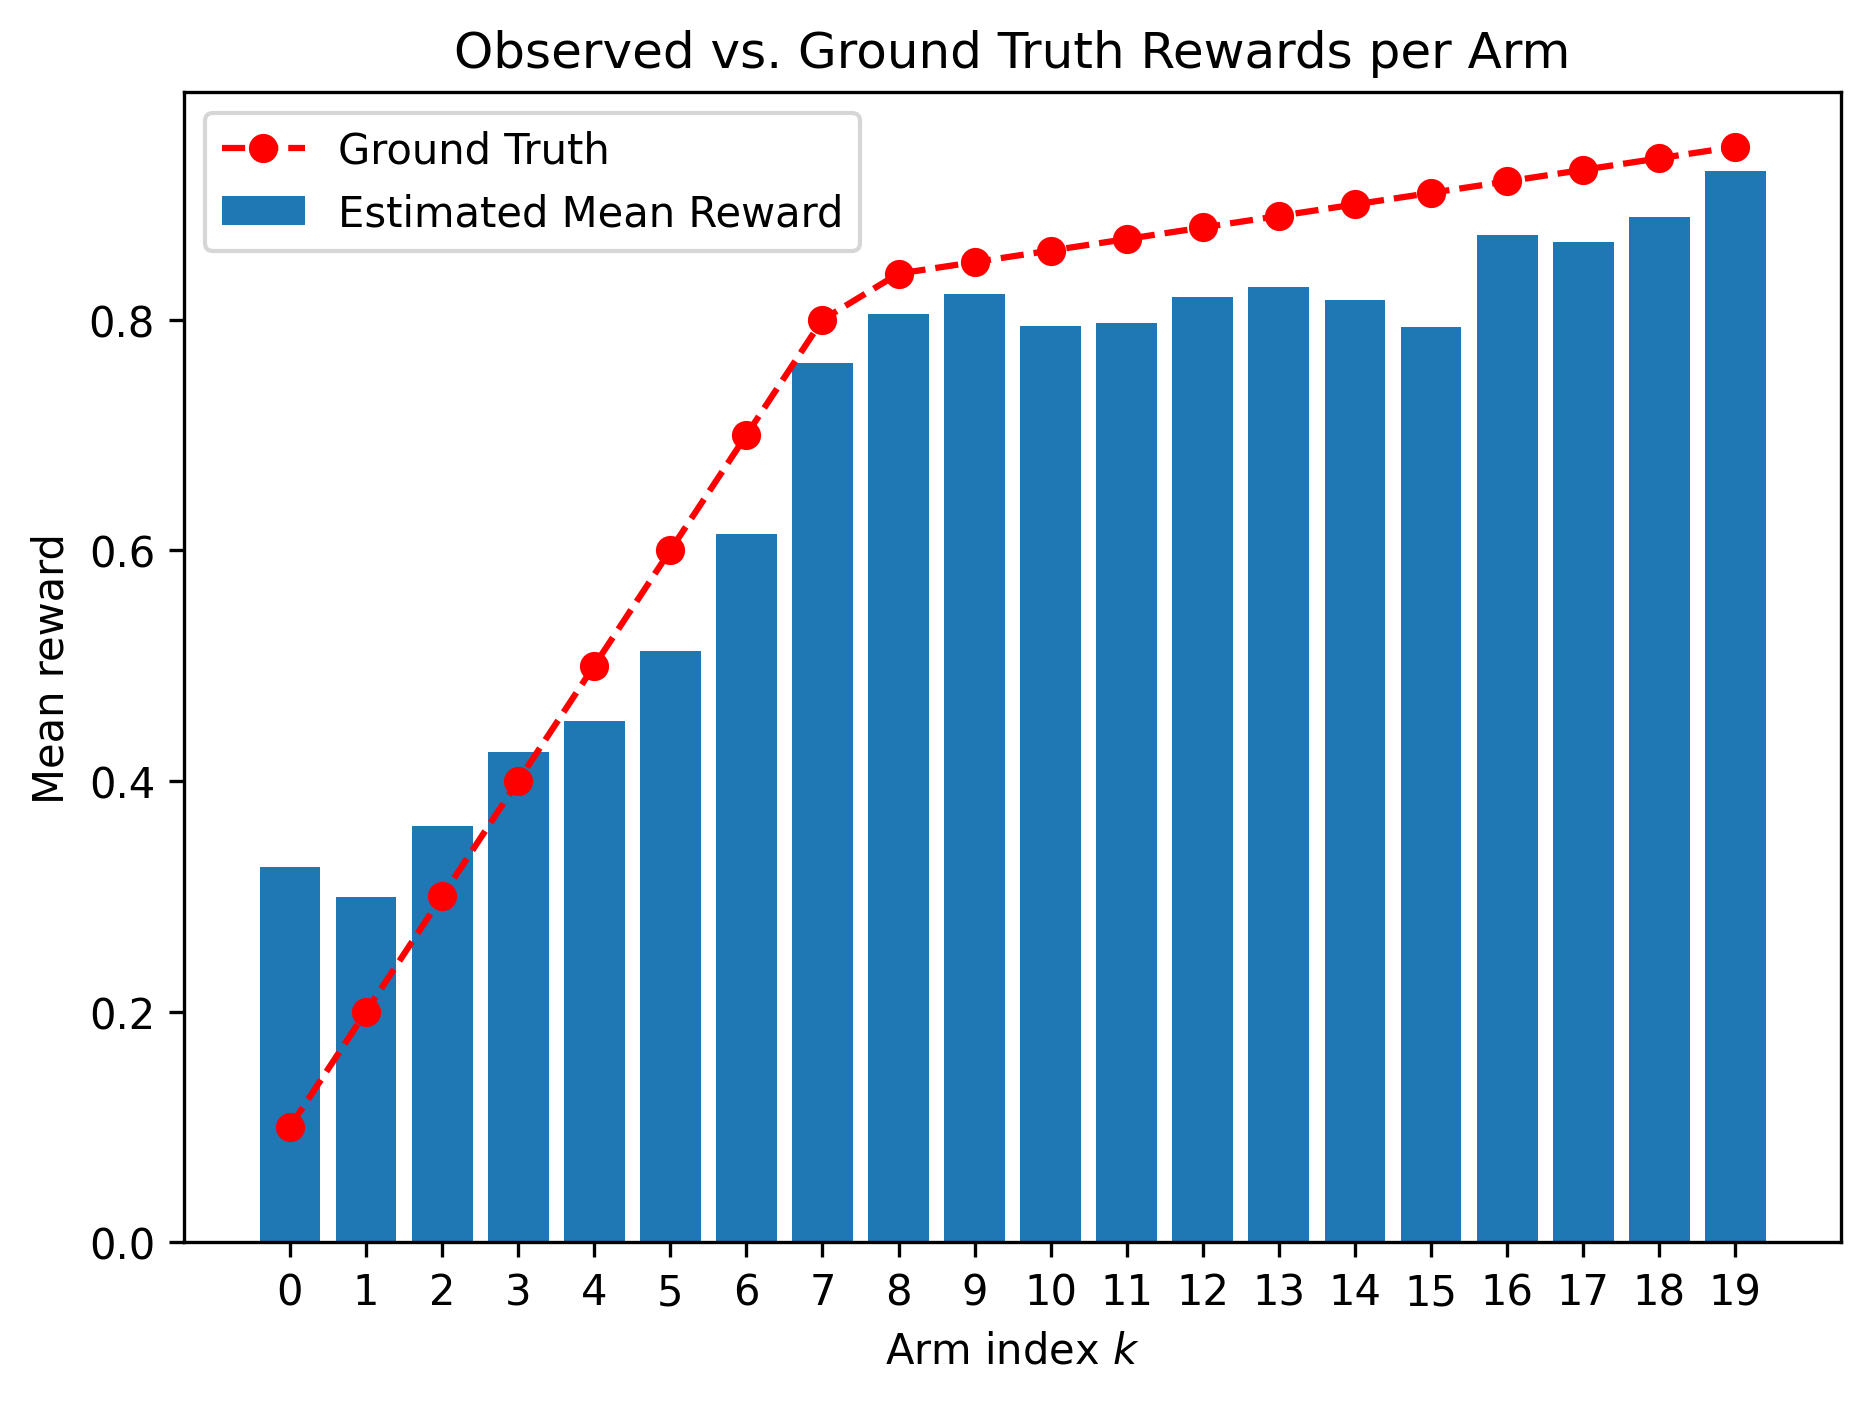
\includegraphics[width=0.48\textwidth]{./Img/stochastic_bandit/reward.png}
    \caption{Left: number of times each arm was selected in the generated trajectories. Right: empirical mean reward for each arm (blue bars) versus its true expected reward (red dashed line).}
    \label{fig:distribution}
\end{figure}
